\chapter{Arduino Startup}
\chaplabel{arduino}

\section{Introduction}
This chapter gives the students an introduction to the hardware we are using and gets them started with 
the Arduino IDE.

\section{Datasheets}
\subsection{Arduino Nano Connect RP2040}
The data sheet for the Arduino Nano Connect RP2040 is located at\\ 
\href{https://docs.arduino.cc/resources/datasheets/ABX00053-datasheet.pdf}{https://docs.arduino.cc/resources/datasheets/ABX00053-datasheet.pdf}.

The main website for it is at \\
\href{https://docs.arduino.cc/hardware/nano-rp2040-connect}{https://docs.arduino.cc/hardware/nano-rp2040-connect}

The pinout is at \\
\href{https://content.arduino.cc/assets/Pinout\_NanoRP2040\_latest.png}{https://content.arduino.cc/assets/Pinout\_NanoRP2040\_latest.png}.

\subsubsection{RP2040 Microcontroller}
The RP2040 microcontroller datasheet (all 654 pages) is at \\
\href{https://datasheets.raspberrypi.com/rp2040/rp2040-datasheet.pdf}{https://datasheets.raspberrypi.com/rp2040/rp2040-datasheet.pdf}.

If you are ever interested in putting the microcontroller onto a circuit board yourself, there is a reference design at \\
\href{https://datasheets.raspberrypi.com/rp2040/hardware-design-with-rp2040.pdf}{https://datasheets.raspberrypi.com/rp2040/hardware-design-with-rp2040.pdf}.

\subsubsection{IMU - ST LSM6DSOXTR}
The IMU datasheet is at \\
\href{https://www.st.com/resource/en/datasheet/lsm6dsox.pdf}{https://www.st.com/resource/en/datasheet/lsm6dsox.pdf}

\subsubsection{Mic - ST MP34DT06JTR}
The microphone datasheet is at \\
\href{https://www.st.com/resource/en/datasheet/mp34dt06j.pdf}{https://www.st.com/resource/en/datasheet/mp34dt06j.pdf}

The \href{https://www.st.com/en/mems-and-sensors/mp34dt06j.html#sample-buy}{overview page} shows that the microphone is still actively being produced.

\subsubsection{WiFi and Bluetooth - U-blox® Nina W102}
The main page for the wireless unit is at \\
\href{https://www.u-blox.com/en/product/nina-w10-series-open-cpu}{https://www.u-blox.com/en/product/nina-w10-series-open-cpu}.

The datasheet is at \\
\href{https://www.u-blox.com/sites/default/files/NINA-W10\_DataSheet\_UBX-17065507.pdf}{https://www.u-blox.com/sites/default/files/NINA-W10\_DataSheet\_UBX-17065507.pdf}.

\subsubsection{Cryptographic IC - Microchip® ATECC608A}
Note that Microchip \href{https://www.microchip.com/en-us/product/ATECC608A}{doesn't suggest using this chip in new designs} so expect that some future versions of the
Nano RP2040 Connect to use the successor (\href{https://www.microchip.com/en-us/product/ATECC608B}{ATTECC608B}).

The datasheet for the 608A is here: \\
\href{https://ww1.microchip.com/downloads/en/DeviceDoc/ATECC608A-CryptoAuthentication-Device-Summary-Data-Sheet-DS40001977B.pdf}{https://ww1.microchip.com/downloads/en/DeviceDoc/ATECC608A-CryptoAuthentication-Device-Summary-Data-Sheet-DS40001977B.pdf}.

Note that it says it is a summary datasheet. You have to sign an NDA with Microchip to see the full datasheet.

\subsection{Circuit Board Parts (v0.5)}
\begin{enumerate}
    \item \href{https://datasheets.maximintegrated.com/en/ds/DS18B20.pdf}{DS18B20+ 1-Wire temperature sensor}
    \item \href{https://datasheet.lcsc.com/lcsc/2001041707_GXCAS-GX18B20_C472471.pdf}{GX18B20 1-Wire temperature sensor}
    \item \href{https://www.st.com/resource/en/datasheet/vl6180.pdf}{VL6180 Distance sensor}
    \item \href{https://sensirion.com/media/documents/213E6A3B/61641DC3/Sensirion_Humidity_Sensors_SHT3x_Datasheet_digital.pdf}{SHT31 Temperature and Humidity sensor}
    \item \href{https://ww1.microchip.com/downloads/en/DeviceDoc/21498D.pdf}{TC1047 Analog out temperature sensor}
    \item \href{https://www.ti.com/lit/ds/symlink/ads7142.pdf?ts=1660651868135}{ADS7142 Analog-to-digital converter (ADC)}
    \item \href{https://www.adafruit.com/product/4383}{Adafruit 1.14" 240x135 Color TFT Display + MicroSD Card Breakout - ST7789}
    \item \href{https://www.pololu.com/product/4012}{U3V40FX Voltage regulator}
    \item \href{https://datasheet.lcsc.com/lcsc/2001060933_TMI-TMI8837_C478955.pdf}{TMI8837 Motor controller}
    \item \href{https://datasheet.lcsc.com/lcsc/2012221837_QST-QMC5883L_C976032.pdf}{QMC5883L Compass}
    \item \href{https://www.st.com/resource/en/datasheet/st25dv16k.pdf}{ST25DV16 NFC I2C}
    \item \href{https://datasheet.lcsc.com/lcsc/2106062036_Worldsemi-WS2812B-B-W_C2761795.pdf}{NeoPixels (WS2812)}
    \item \href{https://www.nxp.com/docs/en/data-sheet/PCA9535_PCA9535C.pdf}{PCA9535 I2C GPIO}
    \item \href{https://datasheet.lcsc.com/lcsc/1810191633_SUNLIGHT-SLR0394FG3C5BD-3-5_C225905.pdf}{SLR0394 LED display}
\end{enumerate}

\section{Schematics and PCB}
\begin{landscape}
\begin{figure}[!htb]
	\centering
	%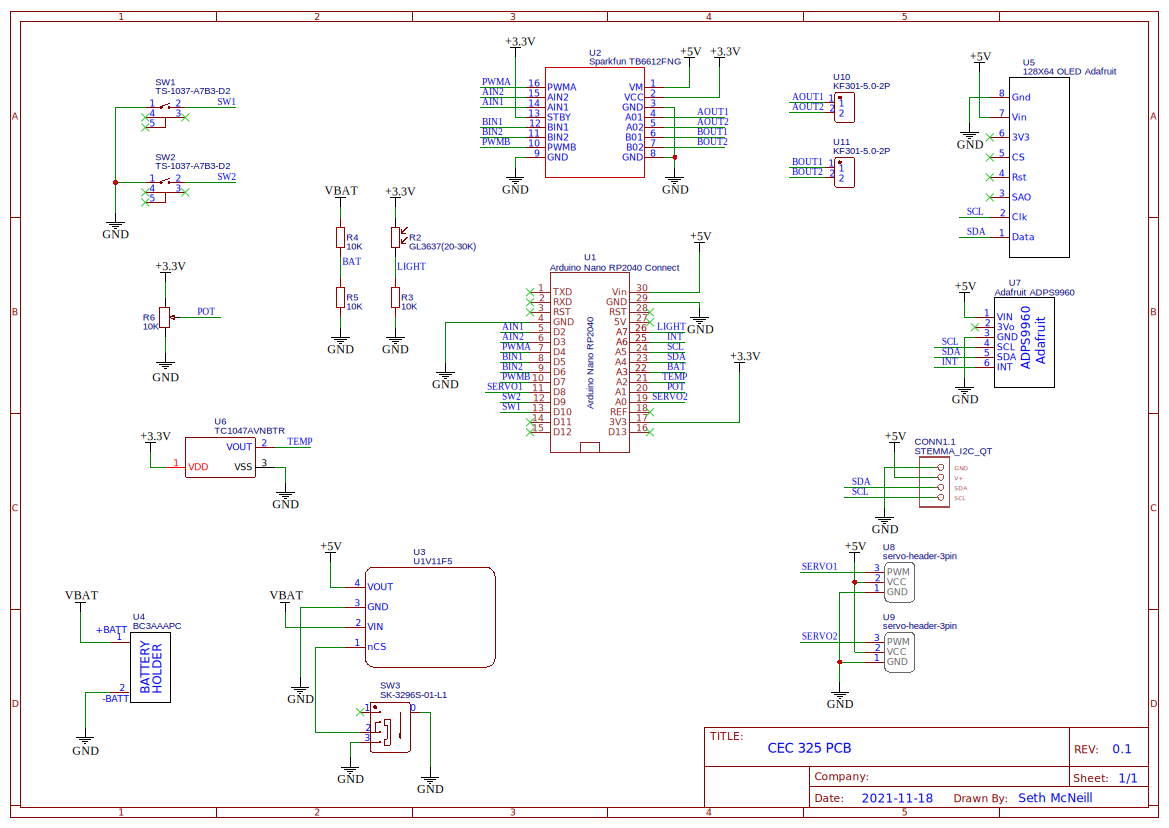
\includepdf[pages=-,pagecommand={},width=\textwidth]{arduinoStart/Schematic_NanoConnectRP2040test1_v0.1.pdf}
	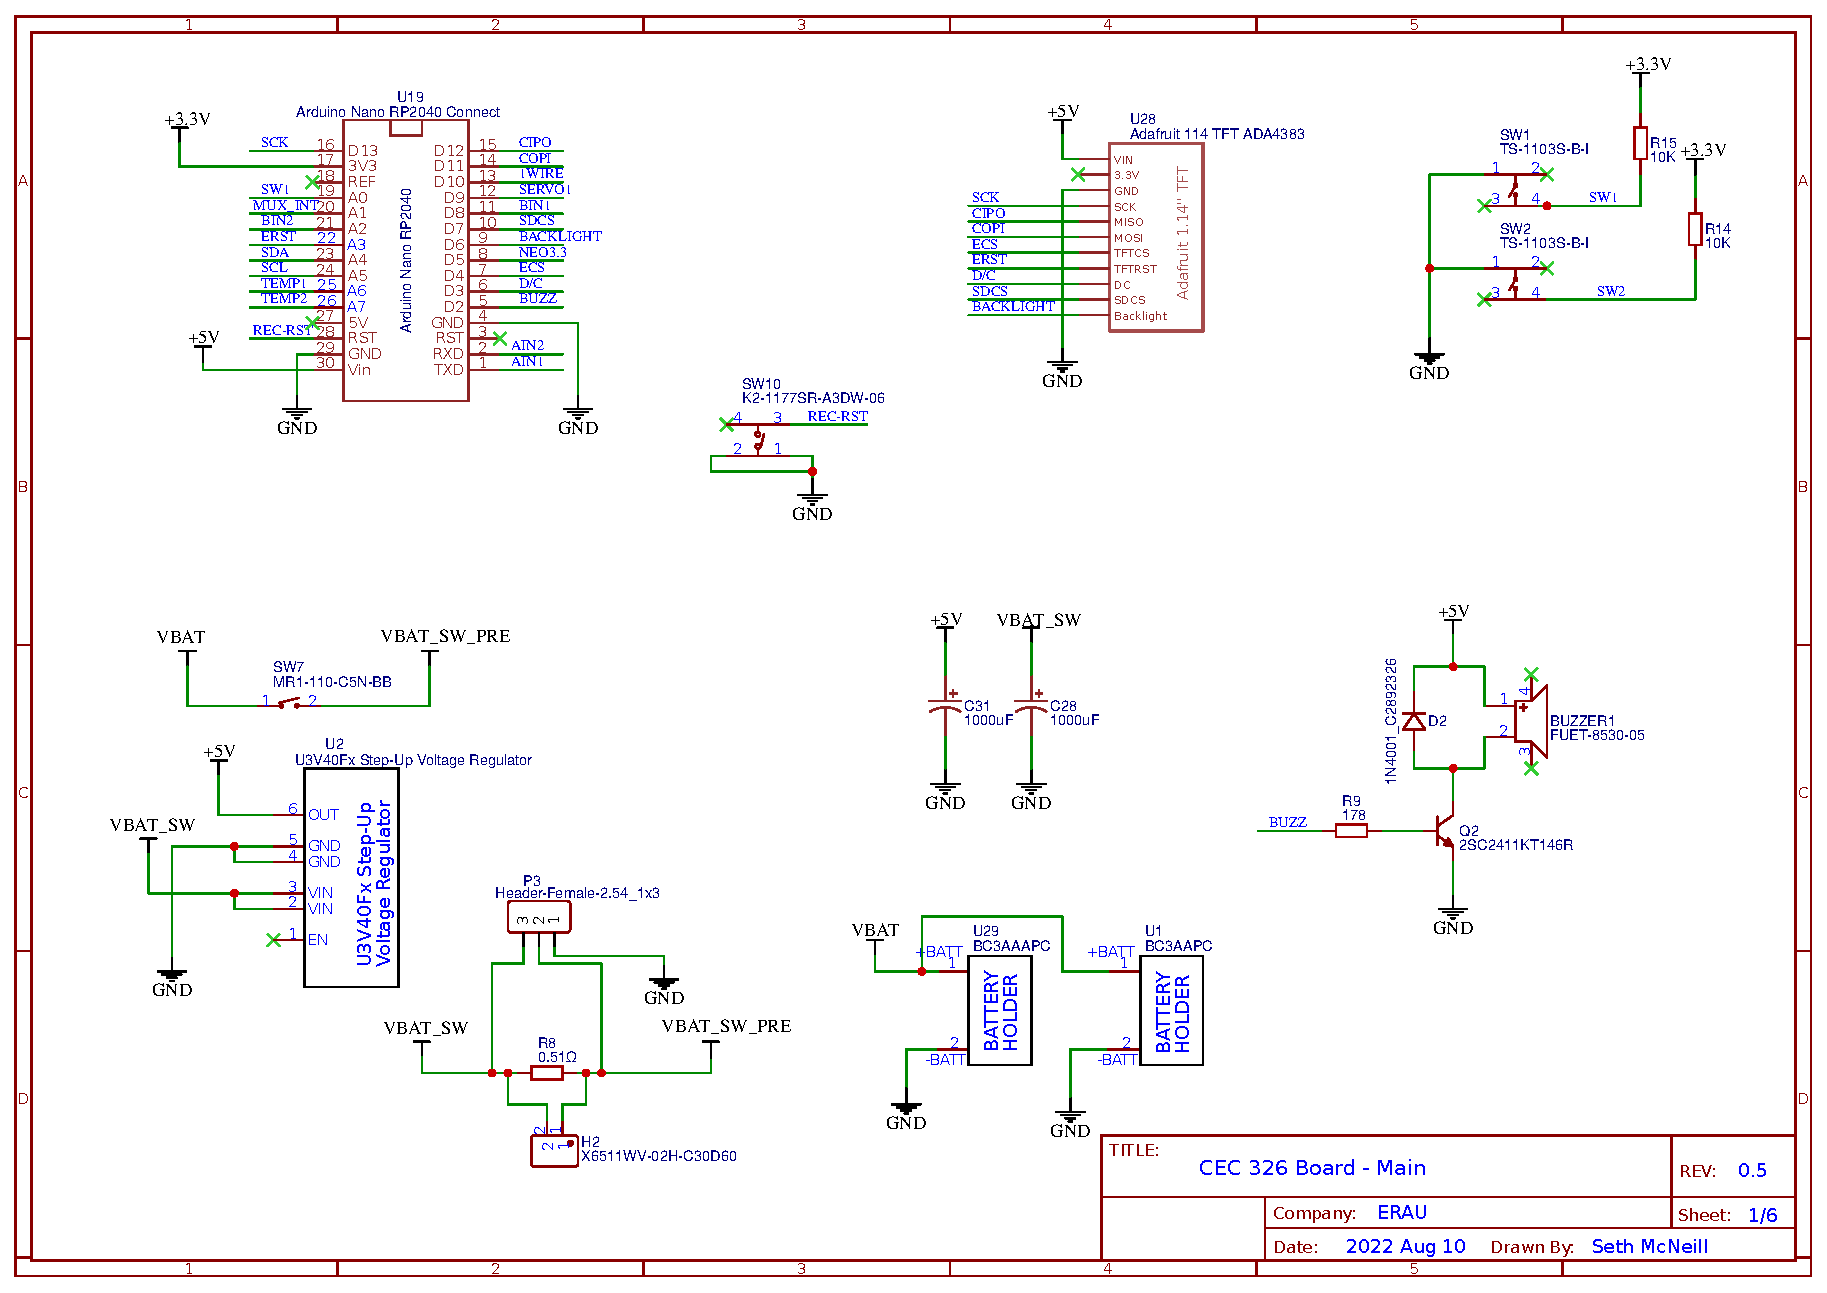
\includegraphics[width=\paperwidth]{arduinoStart/Schematic_CEC326v0.5_Main} % leaving off extension seems to work
	\caption{This is the schematic of version 0.3 of the board. This is the board used in Spring 2022.}
	\label{fig:boardSchematic}
\end{figure} 

\begin{figure}[!htb]
	\centering
	%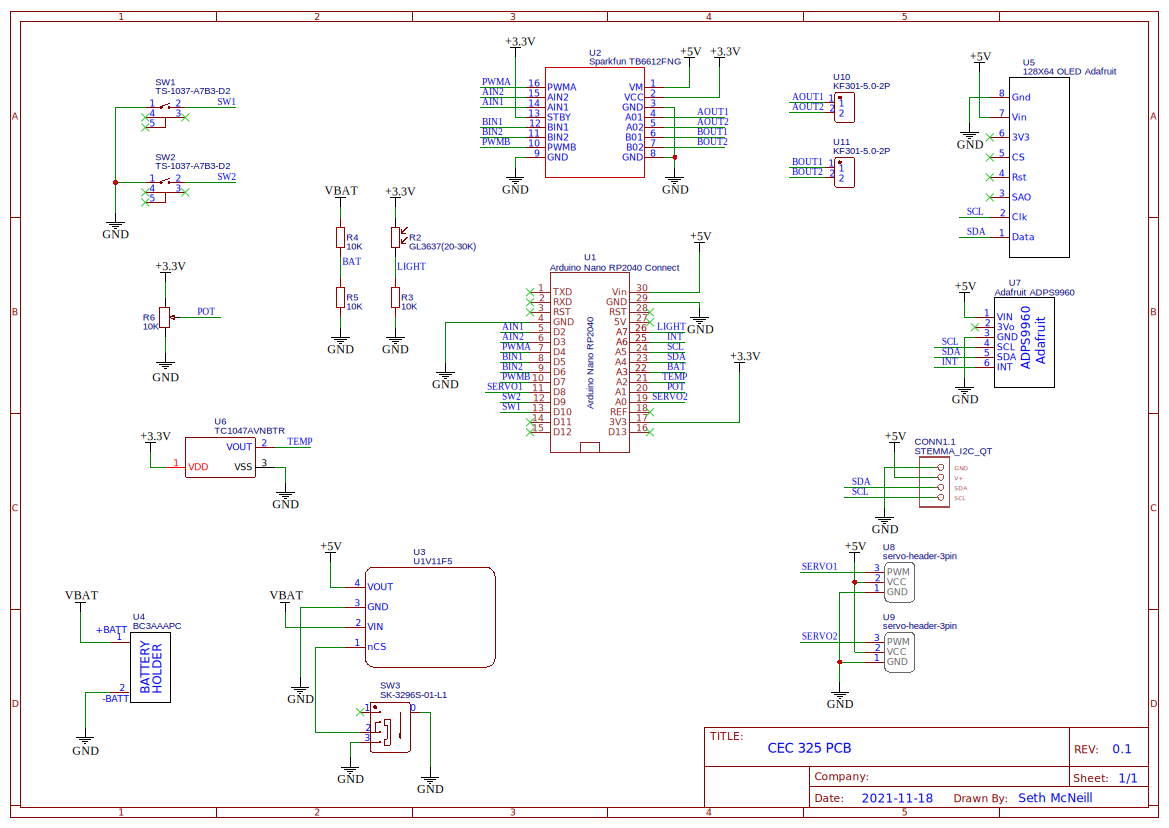
\includepdf[pages=-,pagecommand={},width=\textwidth]{arduinoStart/Schematic_NanoConnectRP2040test1_v0.1.pdf}
	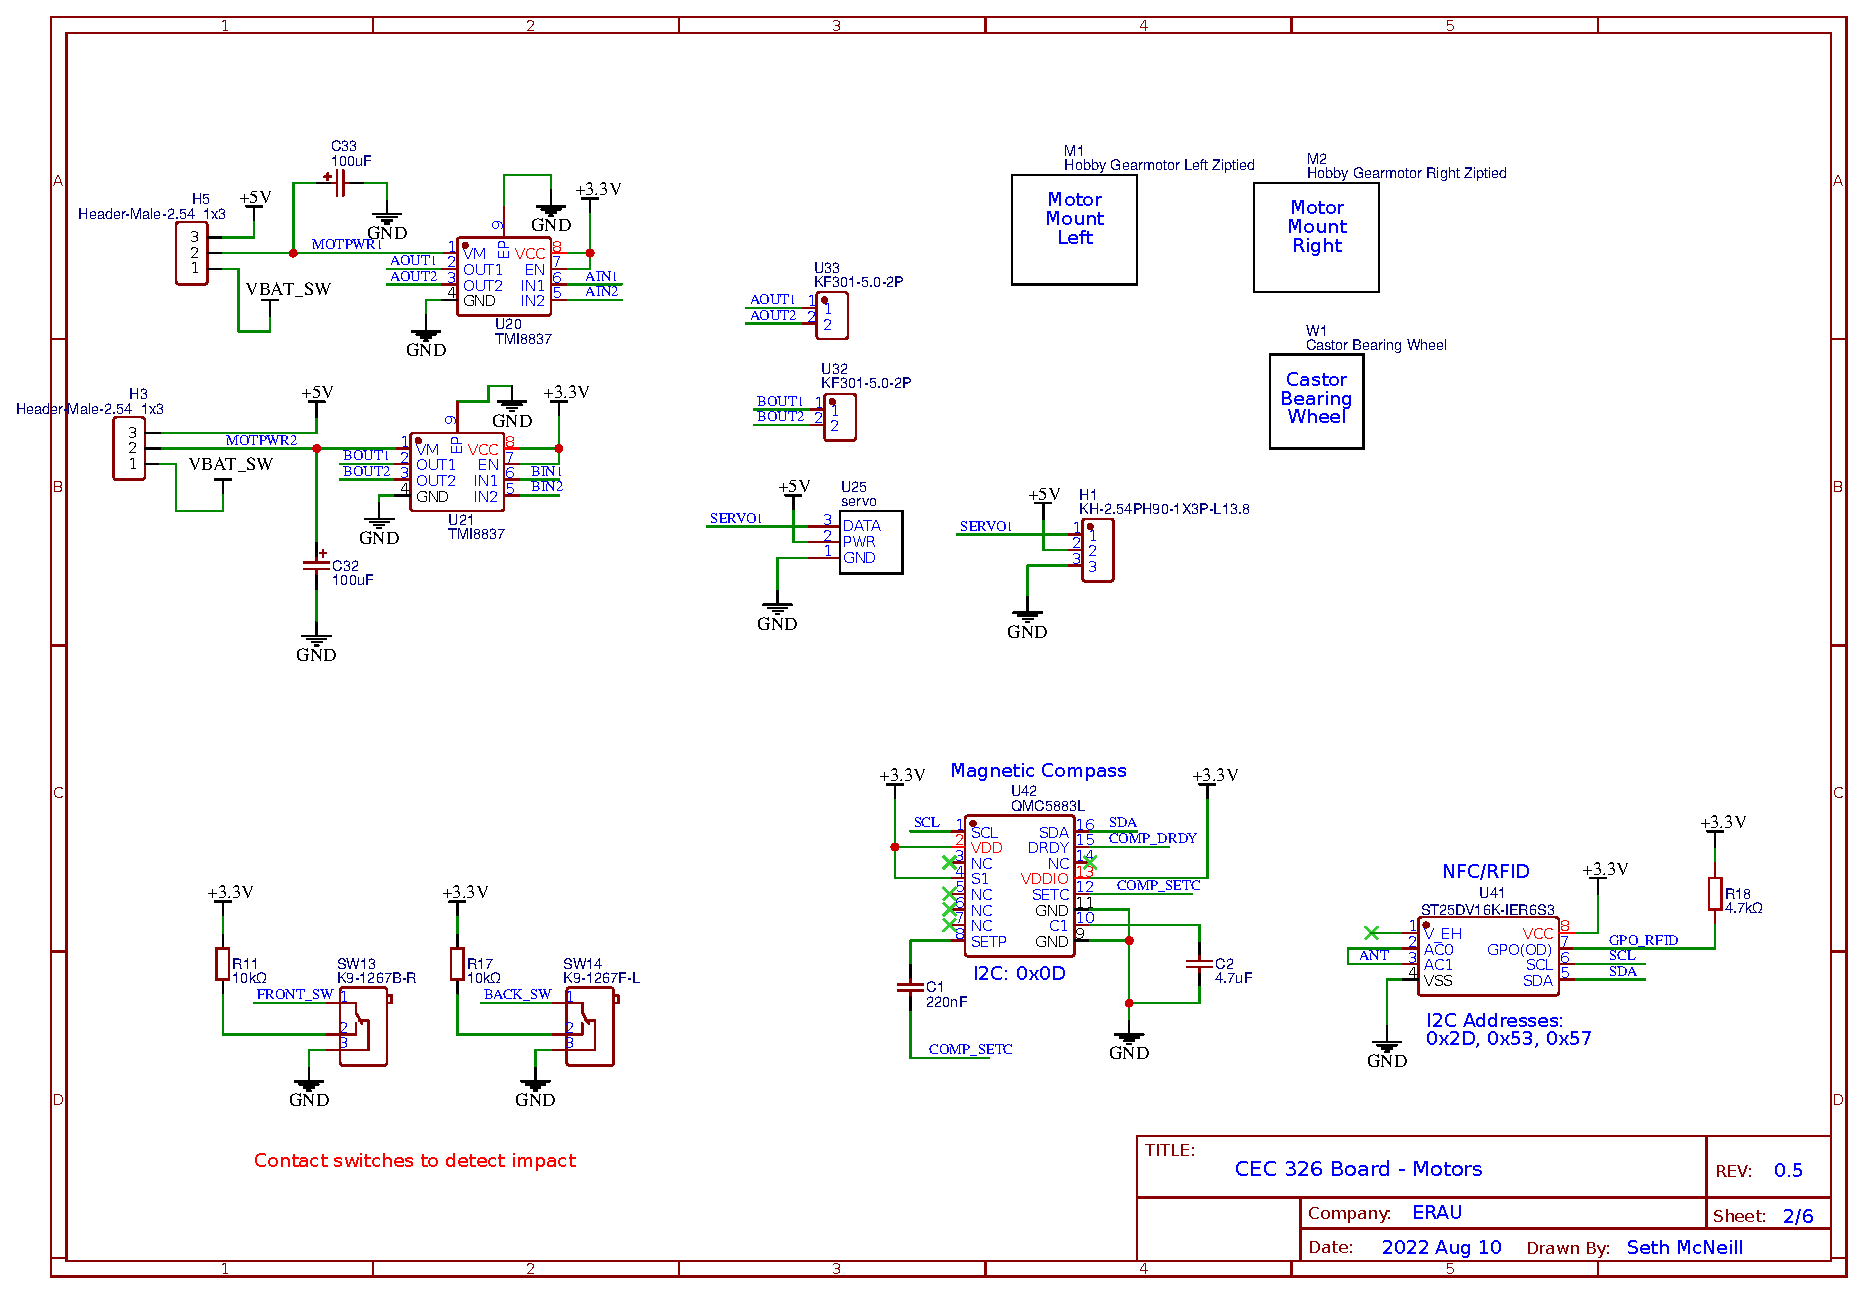
\includegraphics[width=\paperwidth]{arduinoStart/Schematic_CEC326v0.5_Motors} % leaving off extension seems to work
	\caption{This is the schematic of version 0.3 of the board. This is the board used in Spring 2022.}
	\label{fig:boardSchematic}
\end{figure} 

\begin{figure}[!htb]
	\centering
	%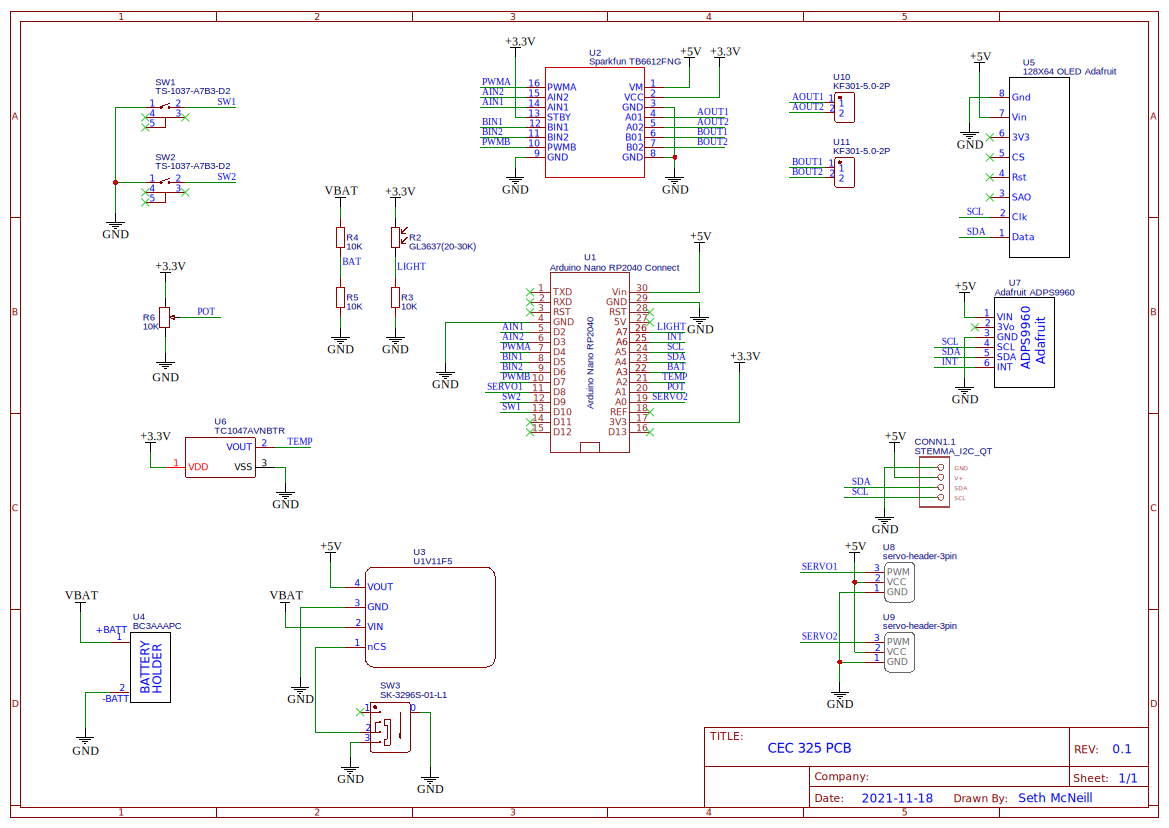
\includepdf[pages=-,pagecommand={},width=\textwidth]{arduinoStart/Schematic_NanoConnectRP2040test1_v0.1.pdf}
	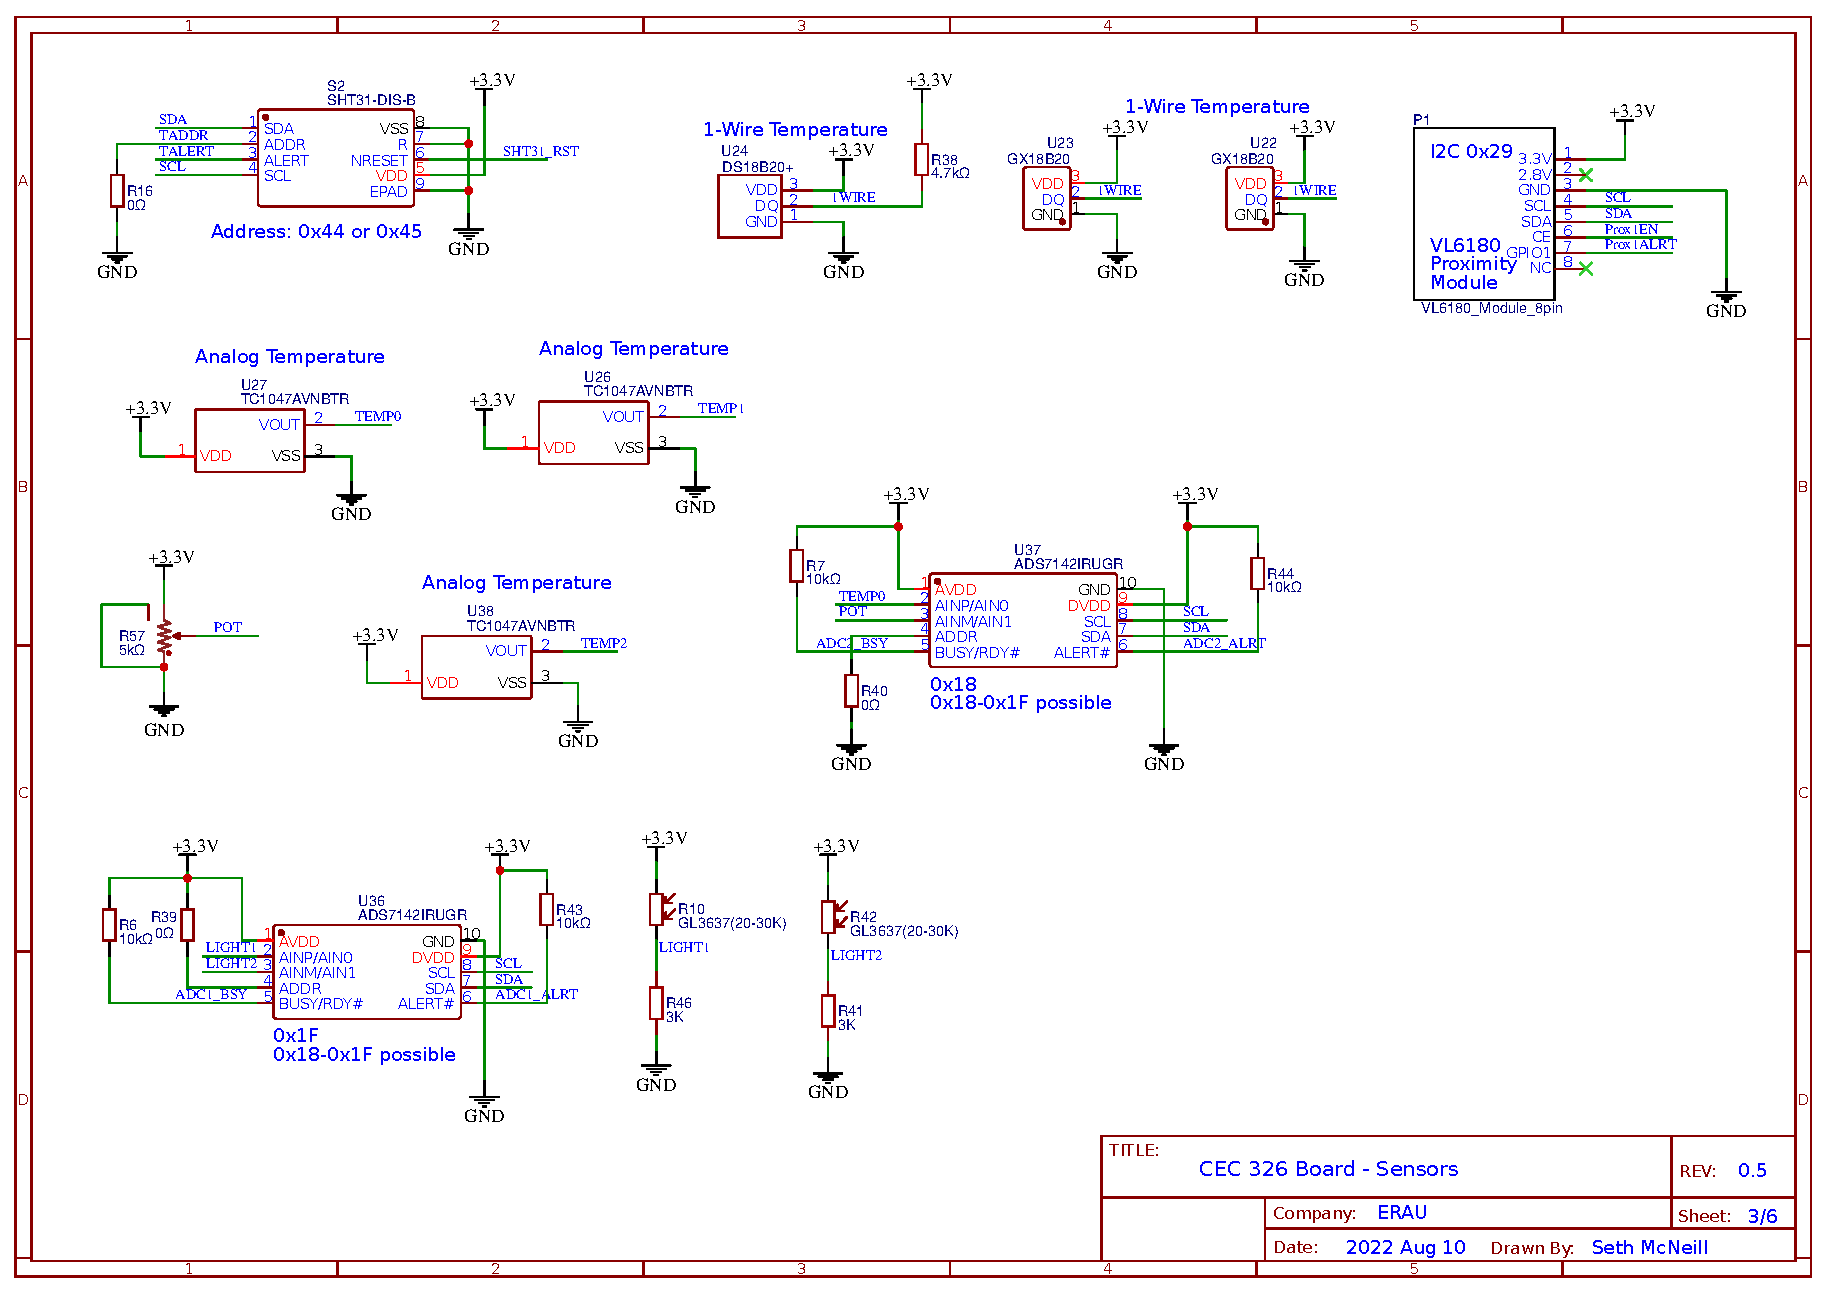
\includegraphics[width=\paperwidth]{arduinoStart/Schematic_CEC326v0.5_Sensors} % leaving off extension seems to work
	\caption{This is the schematic of version 0.3 of the board. This is the board used in Spring 2022.}
	\label{fig:boardSchematic}
\end{figure} 

\begin{figure}[!htb]
	\centering
	%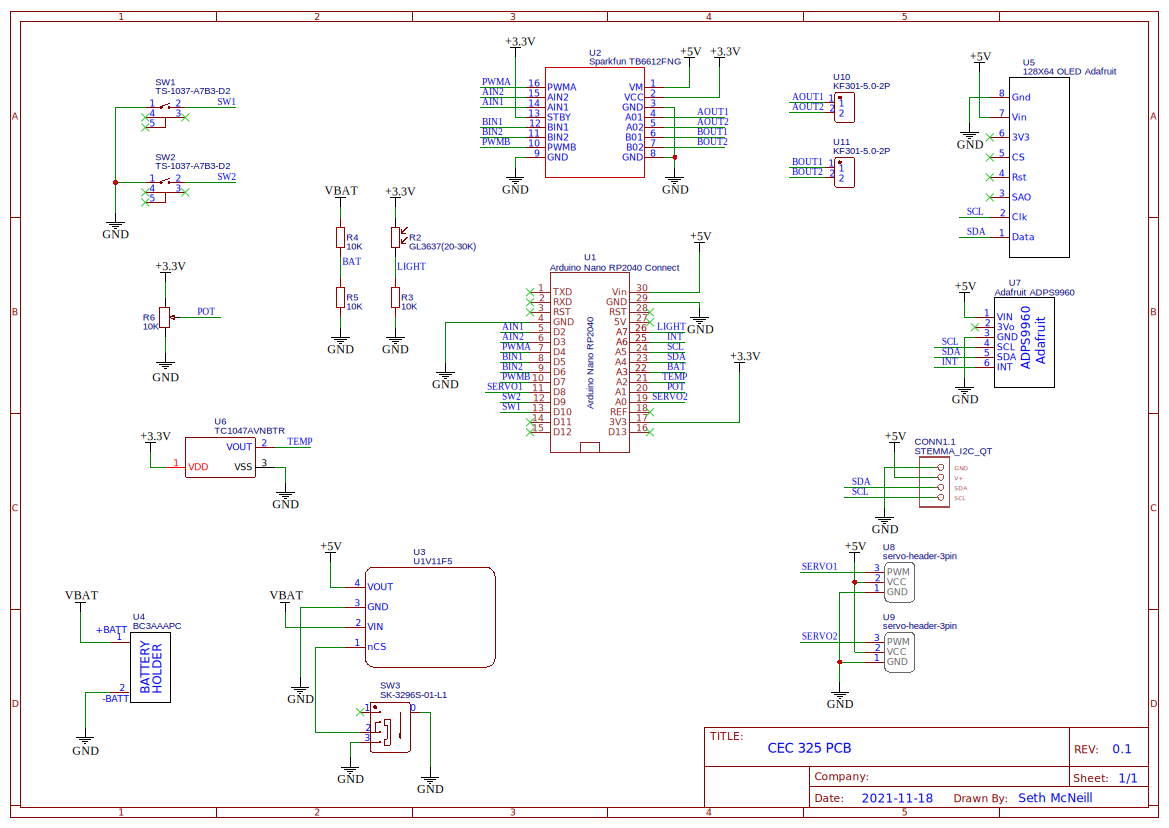
\includepdf[pages=-,pagecommand={},width=\textwidth]{arduinoStart/Schematic_NanoConnectRP2040test1_v0.1.pdf}
	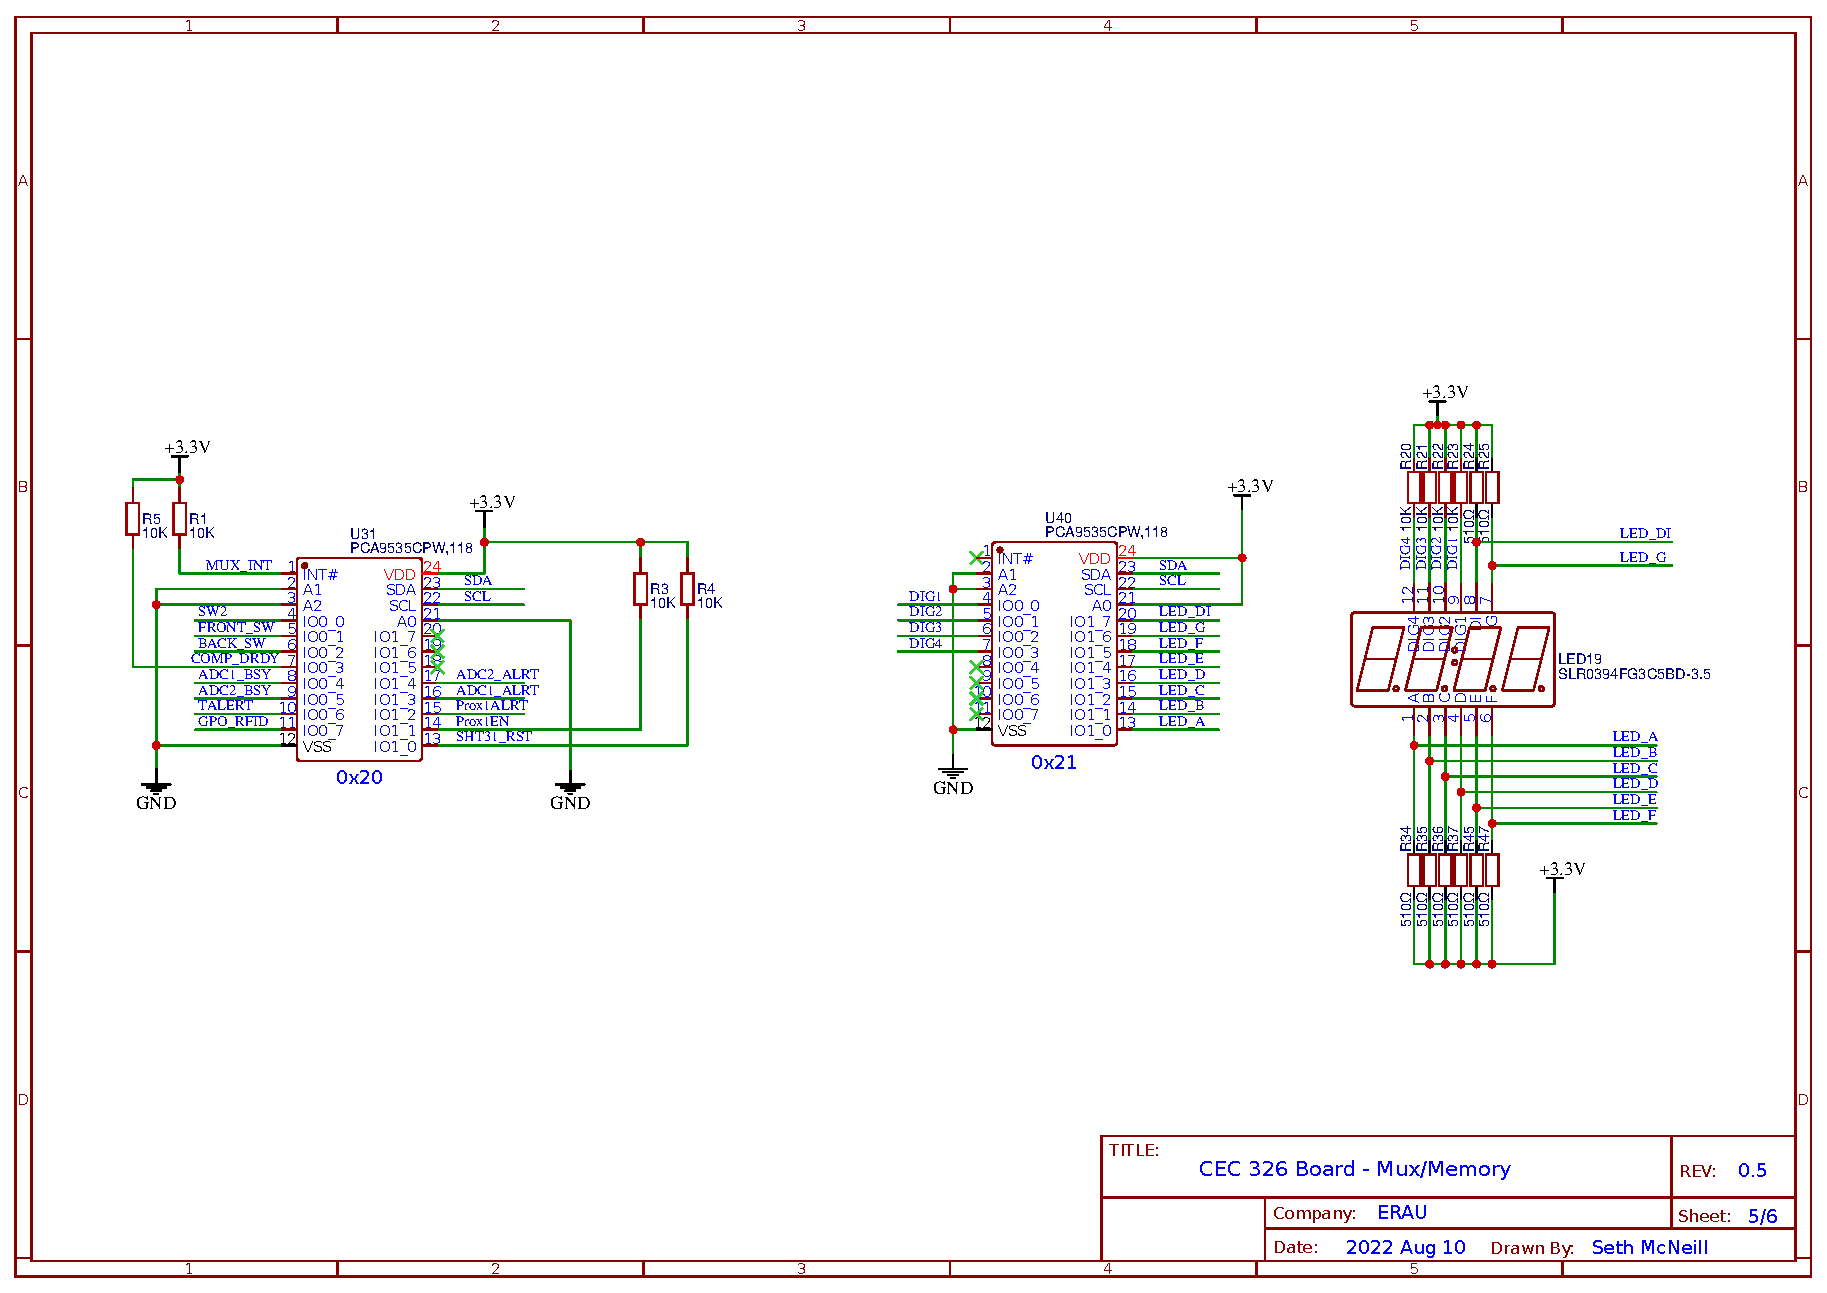
\includegraphics[width=\paperwidth]{arduinoStart/Schematic_CEC326v0.5_Mux} % leaving off extension seems to work
	\caption{This is the schematic of version 0.3 of the board. This is the board used in Spring 2022.}
	\label{fig:boardSchematic}
\end{figure} 

\begin{figure}[!htb]
	\centering
	%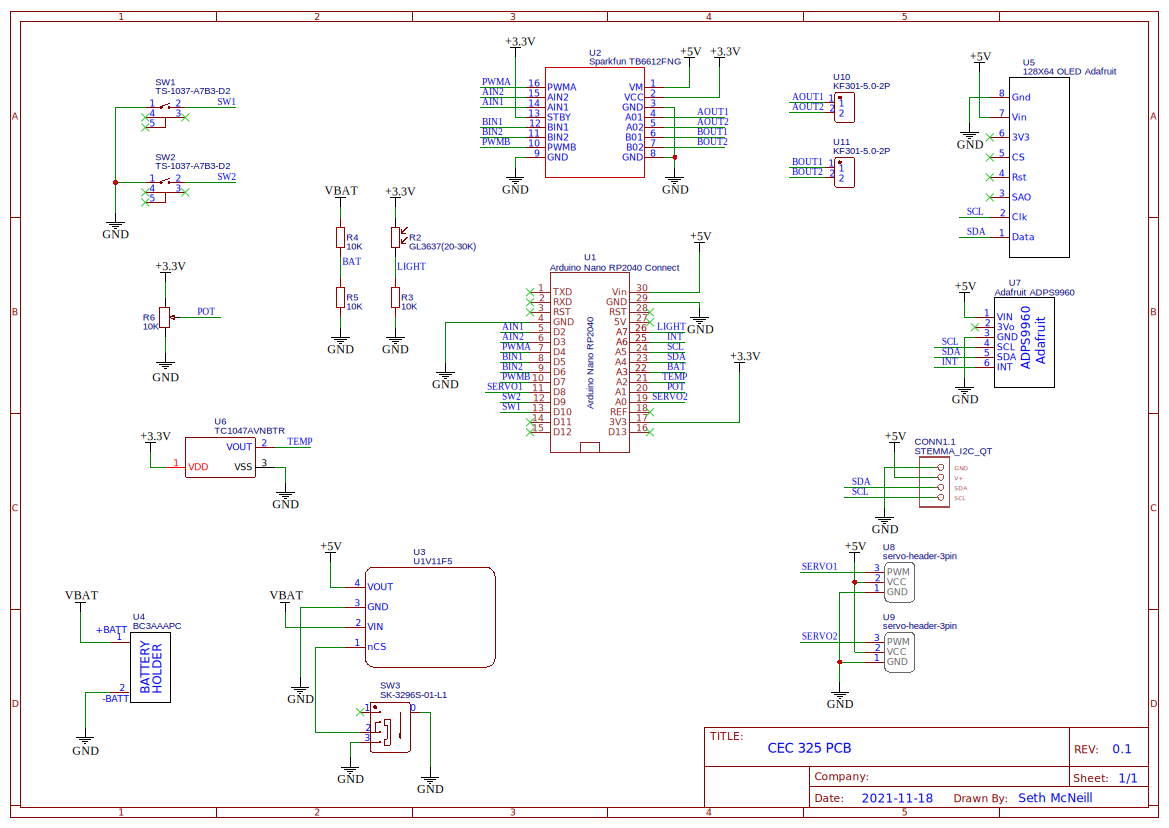
\includepdf[pages=-,pagecommand={},width=\textwidth]{arduinoStart/Schematic_NanoConnectRP2040test1_v0.1.pdf}
	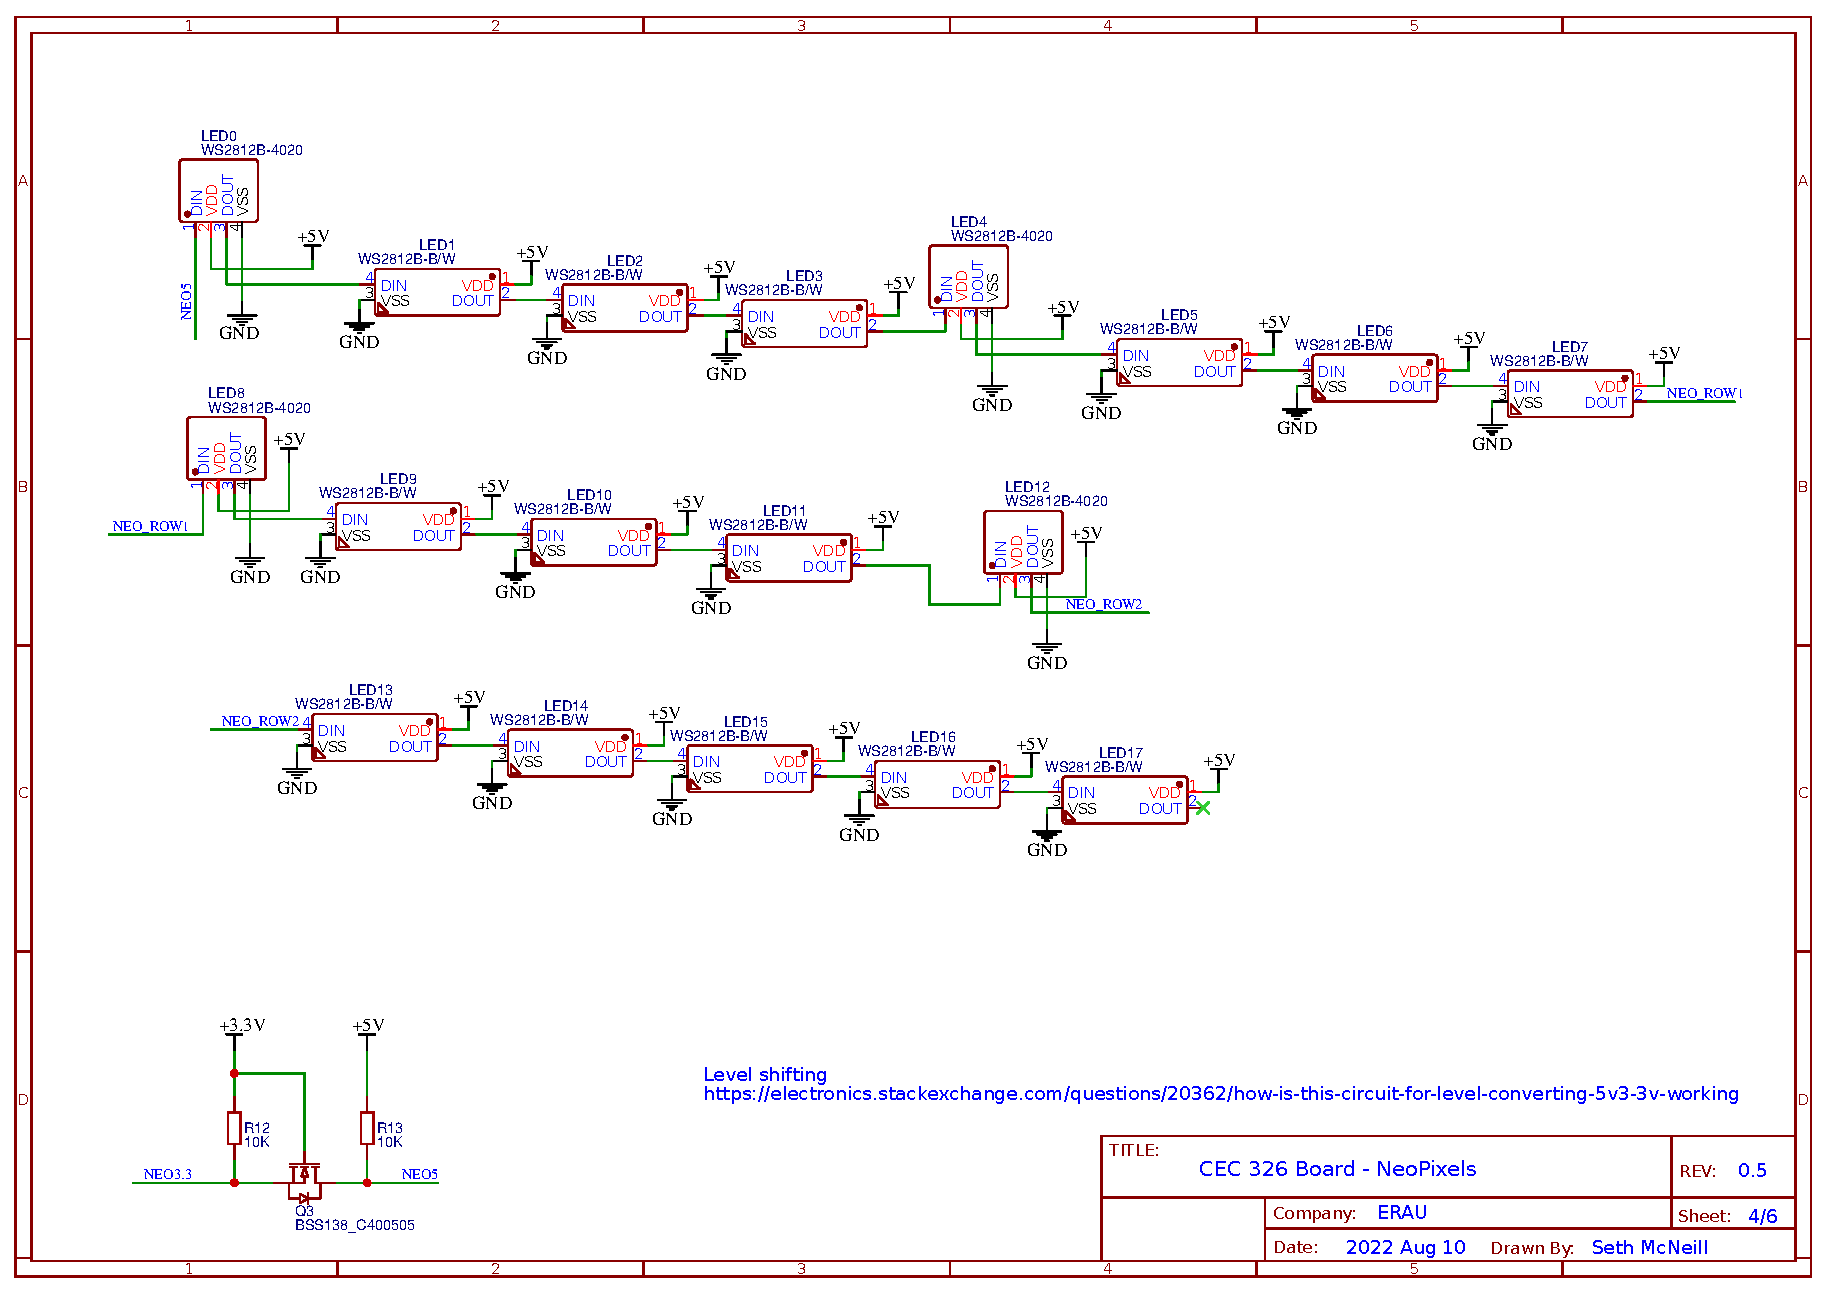
\includegraphics[width=\paperwidth]{arduinoStart/Schematic_CEC326v0.5_NeoPixels} % leaving off extension seems to work
	\caption{This is the schematic of version 0.3 of the board. This is the board used in Spring 2022.}
	\label{fig:boardSchematic}
\end{figure} 

\begin{figure}[!htb]
	\centering
	%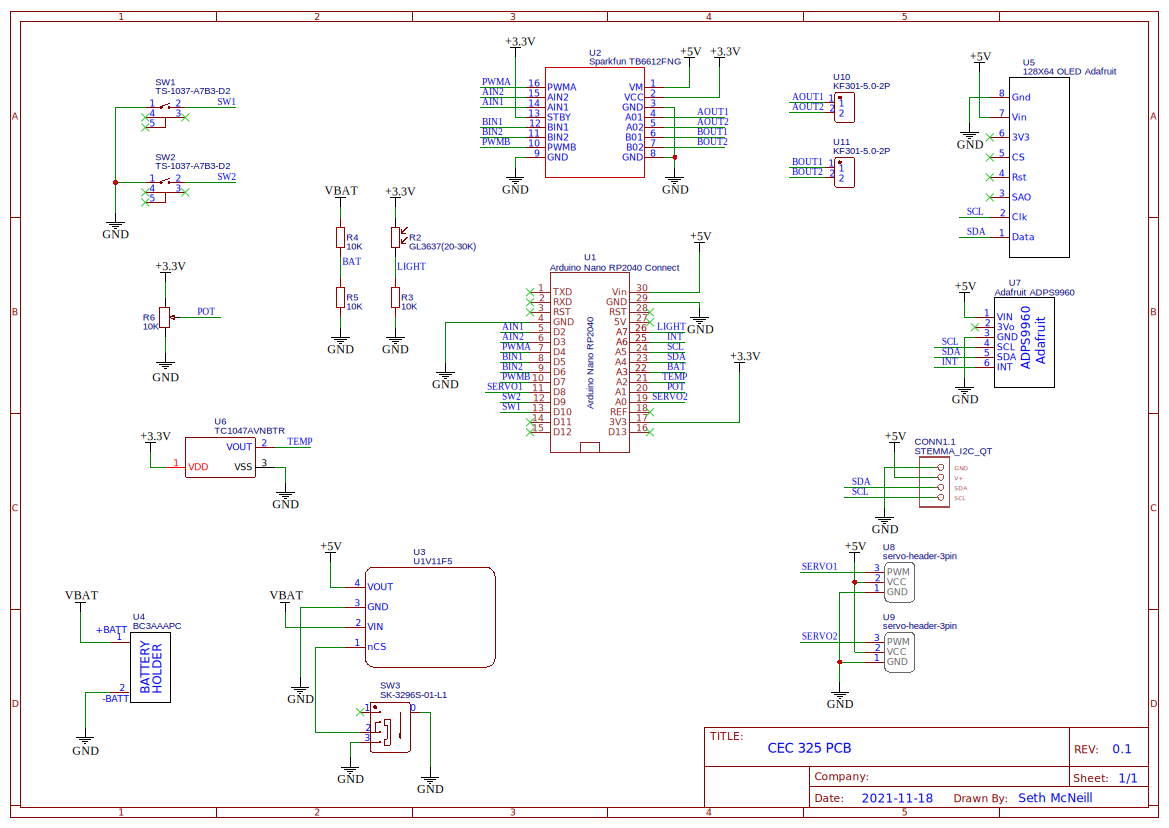
\includepdf[pages=-,pagecommand={},width=\textwidth]{arduinoStart/Schematic_NanoConnectRP2040test1_v0.1.pdf}
	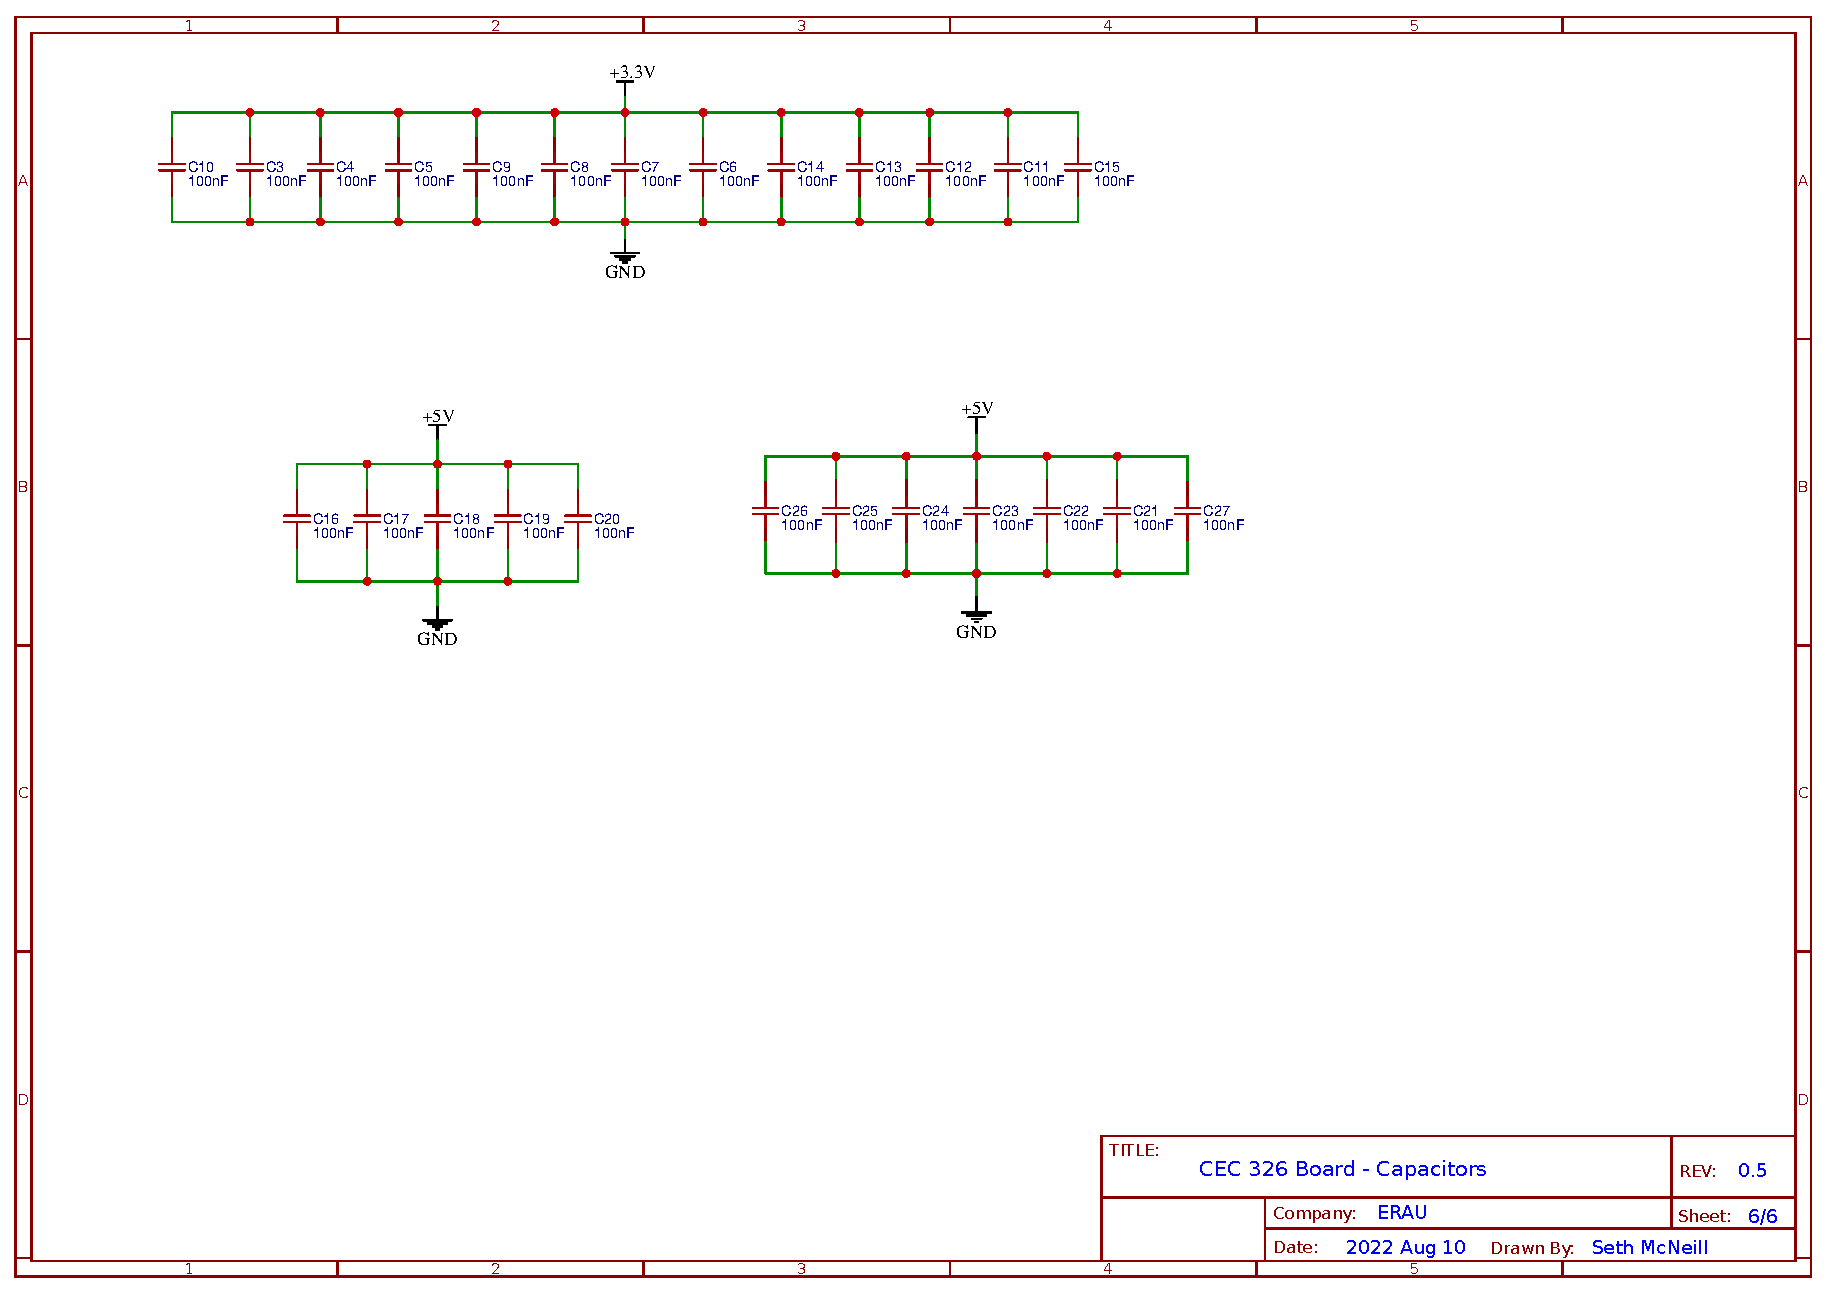
\includegraphics[width=\paperwidth]{arduinoStart/Schematic_CEC326v0.5_Caps} % leaving off extension seems to work
	\caption{This is the schematic of version 0.3 of the board. This is the board used in Spring 2022.}
	\label{fig:boardSchematic}
\end{figure} 

\end{landscape}

\begin{figure}[!htb]
	\centering
	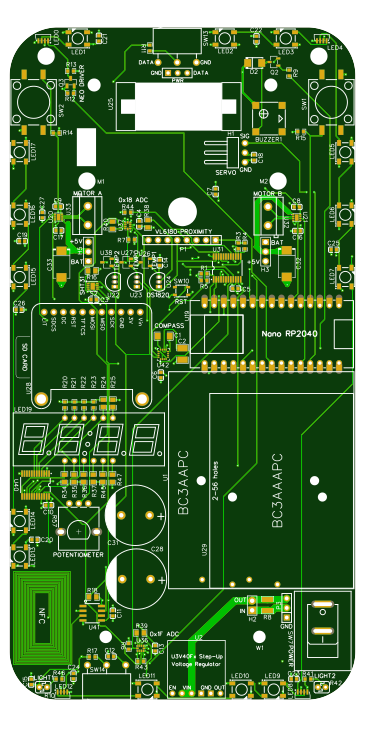
\includegraphics[scale=1.0]{arduinoStart/CEC326v0.5-PCB.png} % leaving off extension seems to work
	\caption{This shows the top of version 0.5 of the board for this class to help locate components.}
	\label{fig:boardTop}
\end{figure} 

